\documentclass{mcmthesis}
\mcmsetup{CTeX = false,   % 使用 CTeX 套装时,设置为 true
        tcn = 55869, problem =  C,
        sheet = true, titleinsheet = true, keywordsinsheet = true,
        titlepage = false, abstract = true}
\problem{C}

\makeatletter % `@' now normal "letter"   %follpw as section test
\@addtoreset{equation}{section}
\makeatother  % `@' is restored as "non-letter"
\renewcommand\theequation{\oldstylenums{\thesection}%
                   .\oldstylenums{\arabic{equation}}}
\newcommand{\upcite}[1]{\textsuperscript{\textsuperscript{\cite{#1}}}}
\usepackage{palatino}
\usepackage{mwe}
\usepackage{graphicx}
\usepackage{tabularx}
\usepackage{float}
\usepackage{indentfirst}
\usepackage{amsmath}
\usepackage{caption}
\usepackage{subfigure}
\title{}
\date{}

\begin{document}

\begin{abstract}%摘要


\title{Keep the Bathtub Warm}



\end{abstract}

\begin{keywords}
	\textbf{A,\indent B, \indent}
\end{keywords}
\maketitle
\tableofcontents\thispagestyle{empty}
%设置页眉
\newpage

\setcounter{page}{1}
%Section 1
\section{Introduction}
\subsection{Literature review}
\indent Traffic flow modeling as the basis of traffic control, traffic design, traffic analysis, traffic simulation and traffic control decision making always is the the research focus in traffic engineering field. And it can be divided into macroscopic and microscopic models from the angle of study, mainly using the theory of fluid mechanics and the theory of car following\upcite{TF1}. Due to their accuracy and practicability, these two models play an important role in the development of traffic flow modeling\upcite{TF2}.\\
\indent The cellular automata (CA) is a kind of grid dynamical model in which time, space and state are discrete, and the space interaction and time causality are local. It has the ability to simulate the spatio-temporal evolution process of complex systems. The study of single lane traffic flow cellular automaton model began in 1986, the most famous of them is the NS model proposed by Nagel and Schreeckenberg in 1992\upcite{ca1}. However, this model has a great flaw, and has been gradually improved by follow-up scientists. Such as the T2 model\upcite{ca2} put forward by Takayasu and the VDR model\upcite{ca3} put forward by barlovic. Cellular automata is now always used to calculate traffic flow problems.\\


\section{Assumptions}
\noindent
{\bf (1) } \textbf{example.} example.\\

\section{Symbols}
\begin{table}[H]
        \setlength{\abovecaptionskip}{0pt}
        \setlength{\belowcaptionskip}{0pt}
				\centering{Table 1:Constants}\\
        \begin{tabular}{p{2cm}|p{2cm}|p{7.5cm}|p{1.7cm}}
		\hline
		\rowcolor[gray]{0.9}\bf{Symbol}	&\bf{uint}      &\bf{Meaning}&\bf{value}	\\
		\hline
		${P}''_{v}$		& $hP_{a}$		 & example  &12\\

		\hline
		\end{tabular}
	\end{table}

\begin{table}[H]
        \setlength{\abovecaptionskip}{0pt}
        \setlength{\belowcaptionskip}{0pt}
        \centering{Table 2:Notation} \\
        \begin{tabular}{p{1.8cm}|p{2.2cm}|p{9cm}}
        \hline
        \rowcolor[gray]{0.9}\bf{Symbol}	&\bf{uint}      &\bf{Meaning}\\
        \hline
        $V(h)$			& $m^3  $		 & example \\
        \end{tabular}
        \end{table}

\section{Models}
\subsection{Design of Cellular Automata }
Large quantities of former traffic simulations based on Cellular Automata (CA) indicate that CA model is a feasible and effective method to emulate traffic flow. Space, time and status are all discrete in Cellular Automata. For example, The model abstracts the car into a particle, and time is divided into small units. This feature predigests the simulation process significantly. Besides, the status of a cell is controlled by its neighboring cells following a set of rules, which is much similar to real-life traffic where a car's movement largely depends on its neighboring cars' movements. Therefore, it is rational for us to apply Cellular Automata in solving our problem.
\\
\subsubsection{The data structure of cellular automata}
We set 5 attributes for each car, including the position ($p$), the distance from the front car ($d$), the speed ($v$), the driver's head time ($t$), the type of the car ($k$).\\
\indent The property vector of each car can be expressed as
\begin{equation}
	car_{i}=\left [ p_{i},d_{i},v_{i},t_{i},k_{i} \right ]
\end{equation}
\indent The properties of all the cars can be superimposed and combined into a two-dimensional matrix, the matrix is as follows
\begin{equation}
	Cars=
	\begin{bmatrix}
	   car_{1}\\
	   car_{2}\\ 
	   ...\\ 
	   car_{n}
	\end{bmatrix}
	=
	\begin{bmatrix}
		p_{1},d_{1},v_{1},t_{1},k_{1}\\
		p_{2},d_{2},v_{2},t_{2},k_{2}\\ 
		...\\ 
		p_{n},d_{n},v_{n},t_{n},k_{n}
	\end{bmatrix}
	=
	\left [ P,D,V,T,K \right ]
\end{equation}
where P,D,V,T,K are column vectors.\\

\subsection{Time Headway}
\subsubsection{The Set of Time Headway}

\indent Time Headway (TH) is the time difference between the two adjacent vehicles passing through the same location. In general, the TH is a random value. But when people drive a car, the front car has an emergency brake or deceleration in a very short time, the following car driver can respond only after a certain reaction time. It is easy to cause traffic accidents if the distance between the two cars is two small. So the HT between the two cars needs to be greater than a minimum safety HT. The safety HT is depended on the reaction time of person.\\
\indent The HT of two vehicles is determined by the subjective judgment of the driver. But generally speaking, when the rear car is far away from the front car, the rear car will speed up and make the HT of two cars smaller. When the driver of rear is aware that the HT is too small, as the HT of reality is less than the HT he expected, the driver will slow down and increase the HT between two cars.\\
\indent Then the ratio distribution of the headway of the car needs to be determined. We can know from the previous research\upcite{TH}, when there is a minimum safety HT and crowding, the shift negative exponential distribution(SNED) can well reflect the distribution of the headway of a large number of vehicles.\\
\indent So the random variable follows the SNED model. It means,
\begin{equation}
		F(t)=1-e^{-\frac{t_{i}-\tau }{T-\tau}}
\end{equation}
\indent Where, \\
\indent $T$ is the average Time Headway in a road.\\ 
\indent In traffic flow theory, traffic flow density.\\
\begin{equation}
\begin{split}
 K = \frac{Q}{V}\\
 D_{a}=\frac{1}{K}=\frac{V}{Q}
\end{split}
\end{equation}
\indent Where, \\
\indent $K$ is the traffic flow density;\\ 
\indent $Q$ is the traffic flow;\\
\indent $V$ is the average velocity of vehicles;\\
\indent $D_{a}$ is the average distance of vehicles.\\
\indent Because the average Time Headway is the ratio of the average distance $D_{a}$ to the average velocity $V $,\\
\begin{equation}
	T=\frac{D_{a}}{V}=\frac{1}{Q}
\end{equation}
\indent It means the average distance is the reciprocal of the traffic flow.
\subsubsection{The generation of Time Headway following SNED model}
\indent When the parameters $T, \tau $ in $F(t)$ are obtained, we need to produce a large number of data that follows the SNED.\\
\indent MATLAB can only produce a group of data following the uniform distribution. To produce a group of data following $ F(t_{i})=1-e^{-\frac{t_{i}-\tau}{T-\tau}},t_{i}>\tau $, we consider a random variable, 
\begin{equation}
	t_{i}=F^{-1}(t_{i})=G(u)=\tau-(T-\tau)\cdot ln(1-u)
\end{equation}
\indent $G(u)$ is the inverse function of $F(t)$.\\
\indent When $ u \sim U(0,1) $, for some constant number $t_{0}>\tau$,\\
\begin{equation}
\begin{split}
	P\{t_{i}\leqslant t_{0}\}&=P\{\tau\leqslant t_{i} \leqslant t_{0} \}\\
&=P\{ G^{-1}(\tau)\leqslant u \leqslant G^{-1}(t_{0})\}\\
&=\int_{G^{-1}(\tau)}^{G^{-1}(t_{0})}f(u)du\\
&=\int_{F(\tau)}^{F(t_{0})}f(u)du\\
&=\int_{F(\tau)}^{F(t_{0})}1du=F(t_{0})-F(\tau)
\end{split}
\end{equation}
\indent Because the minimum Time Headway is $\tau$, $ t_{i} $must be larger than $\tau$ ,so\\
\begin{equation}
	F(\tau)=P{t_{i}<\tau}=0
\end{equation}
\begin{equation}
	P\{t_{i} \leqslant t_{0} \}=F(t_{0})
\end{equation}
\indent It means $t$ follows the SNED $F(t_{0})$.Therefore, the conclusion is obtained that when $ u \sim U(0,1) $, function type random variable follows SNED with parameters $\tau , T $. 
\subsection{example}%TEST
 
\begin{figure}[H]
\centering
\subfigure[When Kp is too small]{
\begin{minipage}{7cm}
\centering 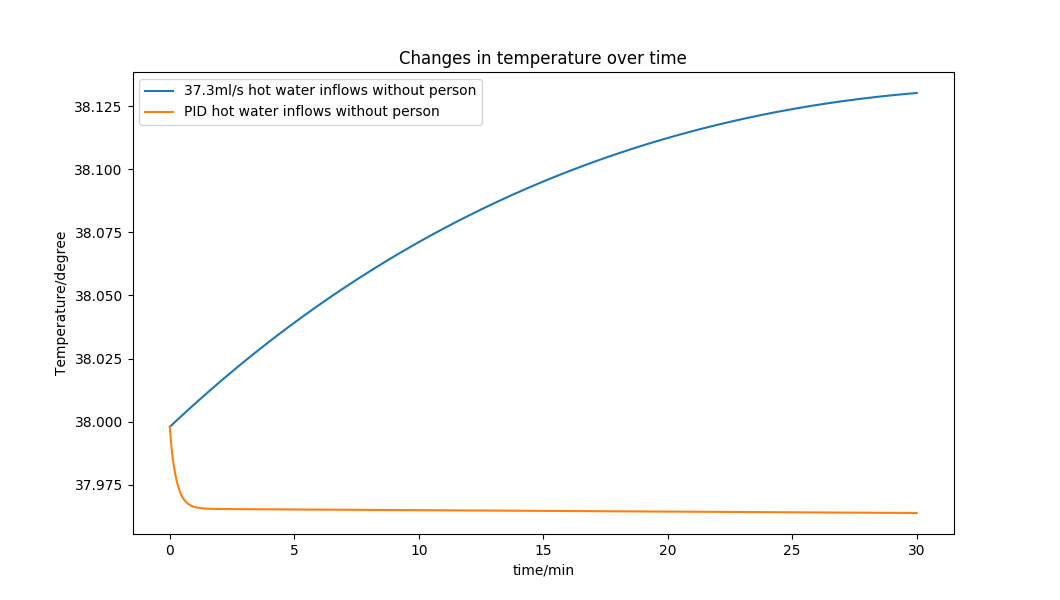
\includegraphics[scale=0.26]{PID_1.png}       
\end{minipage}
}
\subfigure[When Kp is too large]{
\begin{minipage}{7cm}
\centering                                    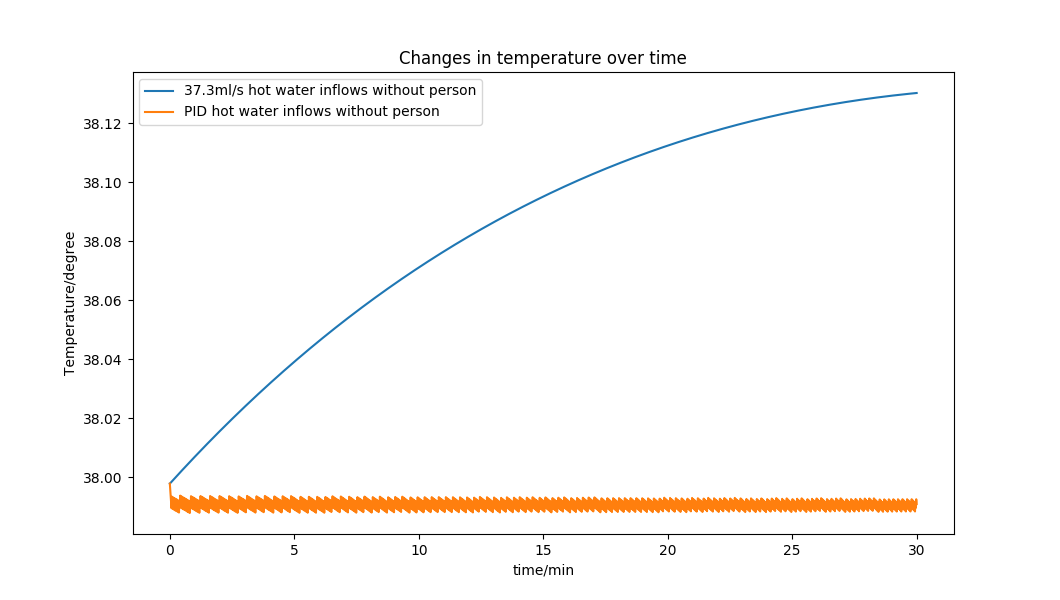
\includegraphics[scale=0.26]{PID_4.png}        
\end{minipage}
}
\caption{Only use Kp\upcite{test}}
\label{PID1}
\end{figure}


\section{Simulation Result and Data Analysis}

\section{Model Validation}

\section{Sensitivity Analysis}

\section{Strengths and Weaknesses}



\section{References}
\begin{thebibliography}{99}
\bibitem{TF1}CREMER M, LUDWIG J. A Fast Simulation Model for Traffic Flow on the Basis of Boolean Operations [J ] . Mathematics and Computers in Simulation, 1986,28(4): 297-303.
\bibitem{TF2}Ding Jian-xun, WANG Ni-shang, SHI Qin. A Two-dimensional BML Model of Traffic Flow Considering Overpass Configuration [ J ]. Journal of Transportation Systems Engineering and Information Technology, 2011,11(6): 98-103
\bibitem{ca1}Nagel K, Schreckenberg M. A cellular automaton model for freeway traffic[ J ].J Phys I : France, 1992,12(2):2221-2229
\bibitem{ca2}Takayasu M,Takayasu H.I/f  noise in a traffic model[ j ]. Fractal -complex Geometry Patterns \& Scaling in Nature \& Society,1996,29(12):3119-3127(9)
\bibitem{ca3}Barlovic R, Santen L, Scnadschneider A. Metas-table states in cellular automate[ J ]. the European Physical Joural B,1998(3): 793-800
\bibitem{ca4}SHI Jun-qing, CHENG Lin, long Jian-cheng, et al.A New Cellular Automaton Model for Urban Two-way Road Networks [ J ]. Computational Intelligence and Neuroscience, 2014,2014;685047
\bibitem{TH}Zhang G, Wang Y, Wei H, et al. Examining headway distribution models with urban freeway loop event data[J]. Transportation Research Record Journal of the Transportation Research Board, 2007, 1999(1):141-149.
\end{thebibliography}



\end{document}